\section{Introduction}
\IEEEPARstart{O}{n} a cast-film line, an agent may read film thickness, compare it with the production target, and propose changing line speed. The thickness measurement and speed setpoint are distinct signals, even if both use Message Queuing Telemetry Transport (MQTT). A runtime that executes such a proposal must resolve it to the correct production context and control node, then decide whether the caller is authorized and the value is admissible. After dispatch, a command receipt is not a setpoint readback, and neither is evidence that film thickness reached its target (Fig.~\ref{fig:control-path}).

Prior work addresses service supervision and skill-based manufacturing~\cite{biskupovic2025supervision,koehle2026llmdriven}, plant-facing semantic grounding and verification~\cite{graul2026aas,schall2026safe}, and multi-agent fault recovery~\cite{vyas2026detection}. We ask how a runtime can connect online acquisition and objective-driven proposals to governed writes without making either protocol access or a task's context a source of write authority. The research contribution is the operation contract that connects these stages, not a new control law or reasoning algorithm.

The runtime separates acquisition from control mappings and read access from write authority. Task-mediated and direct calls share a dispatcher. The write routes recheck approved proposals before dispatch and record command outcomes, readbacks, and later observations separately. The evaluation focuses on the write boundary; it does not establish parity between the two entry paths.

The contributions are:
\begin{enumerate}
  \item A production-scene model that binds operating context, objectives, and limits to direction-specific signal mappings and registered drivers. (Section~III.)
  \item A typed operation path that separates dispatch authorization from value admission and applies approval, revalidation, and evidence recording according to the write route. (Sections~III--V.)
  \item Direct-interface probes and fixtures that assess selected mappings and write rules in simulation, plus exploratory observations from scripted and language-model-driven runs. The tests do not establish parity between task and direct entry paths. (Section~VI.)
\end{enumerate}

\begin{figure}[!b]
\centering
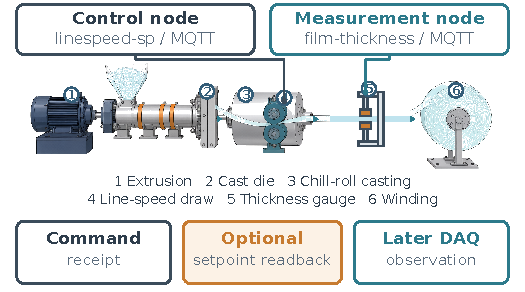
\includegraphics[width=0.98\columnwidth]{resources/fig1-vectorized-20261109.pdf}
\caption{In the cast-film example, the speed setpoint (\texttt{linespeed-sp}) and film-thickness measurement use MQTT but map to distinct nodes. A write produces a receipt and an optional setpoint readback; later film-thickness measurements are separate data-acquisition (DAQ) observations.}
\label{fig:control-path}
\end{figure}


